
\documentclass[12pt]{article}

\usepackage{graphicx}
\usepackage{verbatim}
\usepackage[colorlinks=true]{hyperref}
\usepackage{natbib}

\title{Enabling naturalistic, long-duration and continual animal experimentation}

\begin{document}

\maketitle

\tableofcontents
\pagebreak

\section{Vision}

For over four years, at the Sainsbury Wellcome Centre and Gatsby Computational
Neuroscience Unit, we have been developing the AEON platform, a set of hardware
and software tools that support a new type of experimentation, where animals
are allowed to express ethologically-relevant behaviors, in naturalistic
environments, and in long-duration experiments, while their behavior and
neural activity is monitored continuously for weeks to months.
%
We have used this platform to characterize foraging behavior in both solitary
and groups of mice~\citep{aeonRepo} (Figure~\ref{fig:aeonPlatform}).

Our US partner, the Allen Institute for Neural Dynamics, is using the AEON
platform in continuous learning experiments, where mice freely explore odors
continuously for days to weeks~\citep{carlsPapers}.

This is an unprecedented type of experimentation that \ldots

Several groups around the world are performing this new type of
experimentation~\cite{}.

We have built the AEON platform, and have used it to collect weeks- to
months-long NaLoDuCo experimental data. We next propose to develop advanced
machine learning methods and intelligent visualisations to extract meaning from
this data (Aim 1).

A central aim of both the SWC/GCNU and AIND is to contribute to open science.
We thus propose to create software infrastructure to openly disseminate
NaLoDuCo recordings, visualisation and data analysis methods (Aim 2).

Over more than four years we have developed the AEON platform following high
software engineering practices. It is an open source platform that anybody can
use and modify~\citep{aeonResources}. We want it to become the standard platform for the collection
of NaLoDuCo experimental data.
%
We are currently using AEON on two new NaLoDuCo experiments: (1) odor learning
experiments, lasting for days to weeks, lead by Dr.~Carl Schoonover at the
AIND, and (2) foraging experiments in very large arenas (eight meters in
diameter), lead by Prof.~Tiago Branco at the SWC.
%
We will extend and validate the functionality of the AEON platform by applying
it to these and new NaLoDuCo experiments.
%
A key functionality that we propose to add as part of this project is real-time
machine learning, to allow to control AEON experiments with live inferences
(Aim 3).

\begin{figure}
    \begin{center}
        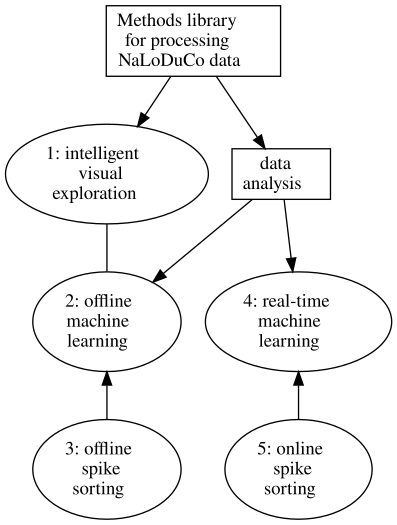
\includegraphics[width=5in]{figures/aims.png}
    \end{center}
    \caption{Proposal aims}
    \label{fig:aims}
\end{figure}

\subsection*{Aim 1: create infrastructure for open dissemination of NaLoDuCo
experimental recordings}

The dissemination of NaLoDuCo recordings is not
trivial, as datasets generated by this new type of experimentation are
enormous. For instance, the size of a dataset generated from a one week
recording of behavioral and neural activity from a foraging mouse in SWC
experiments exceeds 200 terabytes. It will take users several days to download
these datasets over standard Internet connections.

Instead of bringing data to users, we will bring users to data, by storing
datasets in the cloud (or in institutional clusters), and providing
\textbf{cloud software to allow users to visually explore and statistically
analyse behavioural and neural NaLoDuCo datasets where they live}
(Figure~\ref{fig:aims}, left box).

Our statistical analysis of neural time series will require knowledge of the
spiking activity of single units; i.e., spike sorting. In long-duration
experiments with freely moving animals spike sorting is a challenging problem,
because movements of recording probes change the shape of spike waveforms over
time and complicate the assignment of spikes to units based on their waveforms.
We will address this problem by developing \textbf{spike sorting methods for
long-duration and continual, long-duration and high-channel-count recordings}
(Figure~\ref{fig:aims}, left box).

\subsection*{Aim 2: create real-time machine learning methods for intelligent
experimentation}

In small-animal Neuroscience, most often statistical processing of neural time series is
performed offline;
i.e., experimental data is collected, saved to files, which are later
statistically processed, with no runtime constraints. Most often all
experimental data is processes at the same time; i.e., batch processing.

A new online statistical processing approach is now emerging in small-animal Neuroscience,
where data is processes while it is being collected, and at the speed of data
generation~\citep{vermaniEtAl24}.

Online methods are well suited for NaLoDuCo experimentation. In experiments
extending for weeks to months animals learn and adapt, their motivation and
fatigue may fluctuate, and experimental conditions (e.g., lighting) may change.
Offline batch processing algorithms cannot model this type of changing data.
They assume stationary data whose statistical properties do not change across
time. Differently, most online processing algorithms are robust to
these changes.
%
Also, NaLoDuCo experimentation is well suited for online methods, as the
long-duration of these experiments provide a large amount of data to accurately
fit expressive online methods.

We will \textbf{optimize methods developed for Aim~1 so that they can operate
in real time}, and focus on the following two applications of these online
methods (Figure~\ref{fig:aims}, right box).

\subsubsection*{Intelligent neuromodulation}

Brain activity can be modulated optically, chemically and
electrically~\citep{}.
%
Most commonly this modulations is done at fixed experimental times, or based on
simple behavioral or neural observations.

We will guide optogenetic manipulations based on inferences from advanced
machine learning methods.
%
For example, a scientists may hypothesize that a peak in a neural latent
variable, inferred from a prefrontal cortex population, signals the moment when
mice decide to begin a foraging bout.  To test this, she runs an online machine
learning model to estimate latent variables from prefrontal cortex activity,
predicting when this peak will occur. She then optogenetically inactivates the
neural population at the forecasted time.  Because inactivation prevented the
mouse from initiating a foraging bout, her hypothesis is supported.

\subsubsection*{Intelligent experimental data storage}

As the duration of NaLoDuCo experiments become longer, and the richness of the
behavioral and neural recordings become larger, it will be unfeasible to
store all raw data. We will be forced to intelligently decide, in real time,
subsets of data to discard.

For instance, if we are recording videos from a mouse foraging in a large arena
with ten high-resolution cameras, it would save considerable storage if at any
time we only save videos from cameras capturing the mouse at that time.  This
could be done by tracking the position of the mouse in real time with
probabilistic machine learning methods. Then, when the confidence of the
tracking is high, we would only save videos of cameras capturing the mouse at
the tracked position, but when the confidence is low, we would save all videos.

\section{Approach}

We have collected unprecedented NaLoDuCo datasets at the SWC. However, these
very large datasets are of not much use without methods for visual exploration
and data analysis. The next section describes methods we will disseminate for
data analysis and Section~\ref{sec:visualExploration} presents those for
visualisation.

\subsection{Offline analysis methods}

We will disseminate an open-source library of advanced statistical methods
adapted to \textbf{efficiently} process \textbf{non-stationary} recordings from
NaLoDuCo experiments.
%
We will benchmark the performance of these methods for processing behavioral
and neural time series recorded from the SWC NaLoDuCo foraging experiments.

The initial list of methods in this library is given in
Section~\ref{sec:methodsToDisseminate} and includes regression, classification,
supervised, unsupervised and reinforcement learning, state space models and
artificial neural networks.
%
Implementations of these methods will follow high software engineering
standards, and will include detailed documentation, so that users can easily
apply them to process their own NaLoDuCo datasets.
%
If a user needs a machine learning method to process NaLoDuCo recordings not
included in the library, she could use implementations of similar algorithms
included in the library, and their corresponding documentation, to adapt this
algorithm to efficiently process her recordings.
%
This library should be built for all and by all, and become essential to the
rapidly expanding community of scientists performing NaLoDuCo experimentation
in small animals around the world~\citep{}.

In Neuroscience we don't have methods to characterise long-duration and
continual time series, to learn from time series whose statistical properties
fluctuate over time, to forecast time series of long horizons (e.g., hours,
days, week or months.
%
This library should find applicability beyond the realm of small-animal
neuroscience and, for example, be useful to characterize long-duration and
continual neural processes in human brain activity measured with subscalp EEG
electrodes.

\subsection{Initial list of methods}

The first step in the analysis of NaLoDuCo foraging behavioral data is
\textbf{tracking multiple body parts} in mice. For this we will use
\textbf{deep learning} methods, as in
\citep{https://pubmed.ncbi.nlm.nih.gov/30127430/}.
%
Next, we will use the previous tracking outputs to \textbf{infer mice
kinematics} with \textbf{linear dynamical models}, as in
\citep{https://github.com/joacorapela/lds}.
%
We will combine the tracking outputs with the kinematics inferences to
\textbf{infer behavioral states} with \textbf{hidden Markov models}, as in
\citep{https://pubmed.ncbi.nlm.nih.gov/26687221/}.
%
Further, we will \textbf{related kinematics and behavioral states to the
probability of foraging events}, like leaving a patch, with \textbf{generalized
linear models}, as in \citep{}, and \textbf{artificial neural networks}, as in \citep{}.
%
The final step of the behavioral analysis will be to \textbf{infer mice policy
from behavioral measures} with \textbf{inverse reinforcement learning}, as in
\cite{https://arxiv.org/abs/2311.13870v2}.

The characterization of neural data will begin with the \textbf{estimation of latent
variables models}, to reduced the dimensionality of multielectrode recordings of
hundreds or even thousands of neurons to a small number of latent variables,
using \textbf{latent variable models}, with linear~\citep{dunckerAndSahanai18}
and nonlinear~\citep{pandarinathEtAl} latent dynamics..
%
We will use the estimated latent variables as inputs to
\textbf{infer neural states}, using \textbf{HMMs}, as in~\citep{}.
%
Next, we will \textbf{decode mice position} from hippocampal recordings, and
\textbf{study
replay} during long-duration \textbf{foraging}, with \textbf{point process
decoders}, as in \citep{ppDecoder}.

\subsubsection{Challenges}

Extracting meaning from long-duration and continual recordings opens
challenges and opportunities that we will address and exploit in this project,
as we describe in this and the next sections.

\subsubsection*{Non-stationarities}

Conventional offline methods used to characterize neural time series assume
that the statistical characteristics of the modeled data do not change with
time (i.e., that the probability of the data is time invariant --
stationarity). This assumption may be valid for shorter experiments. However,
for long-duration experiments, where animals learn and adapt, where their
motivation fluctuates, and their activity is modulated by circadian, utradiem
and peridiem rhythms, this assumption may not hold.
In nonstationary environments,
a non-adaptive model trained under the false stationarity
assumption is bound to become obsolete in time, and perform
sub-optimally at best, or fail catastrophically at worst.

The field of adaptive signal processing develops algorithms to characterize
non-stationary systems~\citep{haykin02}. In this field adaptations to specific
algorithms have been developed to improve their performance in non-stationary
environments.

For example, the recursive least-squares algorithm \citep[][Chapter
9]{haykin02} is an adaptation of the ordinary least square algorithm to perform
\textbf{linear regression} with non-stationary data.

For non-linear regression using \textbf{artificial neural networks}, a very large number
of strategies have been developed to address data non-stationarity. To mention
a few, continual learning has introduced algorithms like  Elastic Weight
Consolidation~\citep[EWC][]{} and Learning Without Forgetting~\citep[LwF][]{}
to allow models to adapt to changes over time without catastrophic forgetting.
Also from this subfield is the Experience Replay (ER) algorithm that stores
past data samples in a buffer and replays them alongside new data during
training. A different type of strategy is used by ensemble methods~\citep{},
which combine multiple models trained on different time windows to capture
evolving data patterns.

Algorithms for \textbf{state-space models}, like the Kalman filter, perform well in some
simpler non-stationary environments producing Gaussian data with varying mean and
covariance.
%
For more complex non-stationarities one can use switching state-pace models,
like the switching linear dynamical system~\cite{} or the switching Hidden
Markov model~\cite{}, or particle filters~\citep{}.

# RL

# concept drift

In the machine learning literature, non-stationary methods are developed to
address the problem of concept drift. It refers to the phenomenon where the
statistical properties of data change over time, leading to a shift in the
underlying relationships between variables. This presents a significant
challenge for machine learning models, as assumptions made during training may
become invalid, leading to degraded performance.
%
Differently from adaptive signal processing, the methods developed to tackle
concept drift are model agnostic and can be used with multiple machine learning
models.

Concept drift can be categorized into different types based on the nature and
rate of change:

\begin{description}

    \item[Sudden Drift:] A rapid and abrupt change in the data distribution
        (e.g., fraud detection after a major security breach).

    \item[Gradual Drift:] A slow transition from one concept to another over
        time (e.g., changing consumer preferences in e-commerce).

    \item[Incremental Drift:] A continuous and progressive evolution of
        concepts (e.g., aging-related changes in medical diagnosis models).

    \item[Recurring or Seasonal Drift:] Periodic shifts in data distribution
        that return to previous states (e.g., seasonal demand fluctuations in
        retail, temperature variations affecting energy consumption, or annual
        trends in influenza outbreaks).

\end{description}

Detecting and adapting to concept drift is crucial for maintaining model
performance. The primary approaches include:
- **Statistical Tests and Distribution Monitoring:** Methods such as
Kullback-Leibler divergence, Kolmogorov-Smirnov tests, and hypothesis testing
can identify drift by comparing past and present distributions.
- **Windowing Techniques:** Sliding windows, fixed or adaptive, monitor recent
data points and adjust the model accordingly.
- **Ensemble Methods:** Combining multiple models with different levels of
adaptability to mitigate the effects of drift.
- **Online Learning and Incremental Updates:** Continuously updating models
with new data to reflect the latest trends.
- **Drift-Aware Bayesian and Probabilistic Models:** Approaches such as
Bayesian Online Learning allow probabilistic reasoning over changing data
distributions.
- **Unsupervised Drift Detection:** Methods such as clustering evolution,
density estimation changes, and autoencoder-based monitoring can detect drift
without labeled data.

**Concept Drift: A Review**

### 1. Introduction
Concept drift refers to the phenomenon where the statistical properties of data
change over time, leading to a shift in the underlying relationships between
variables. This presents a significant challenge for machine learning models,
as assumptions made during training may become invalid, leading to degraded
performance. Concept drift affects a broad range of learning paradigms,
including **supervised, unsupervised, and reinforcement learning**. In
supervised learning, it impacts predictive models by altering the relationship
between input features and target variables. In unsupervised learning, it
affects clustering, anomaly detection, and density estimation models by
shifting the underlying data distribution. In reinforcement learning,
non-stationary environments can cause learned policies to become suboptimal
over time. Concept drift is particularly relevant in dynamic environments such
as financial markets, healthcare, cybersecurity, and personalized
recommendation systems.

### 2. Types of Concept Drift
Concept drift can be categorized into different types based on the nature and
rate of change:
- **Sudden Drift:** A rapid and abrupt change in the data distribution (e.g.,
fraud detection after a major security breach).
- **Gradual Drift:** A slow transition from one concept to another over time
(e.g., changing consumer preferences in e-commerce).
- **Incremental Drift:** A continuous and progressive evolution of concepts
(e.g., aging-related changes in medical diagnosis models).
- **Recurring or Seasonal Drift:** Periodic shifts in data distribution that
return to previous states (e.g., seasonal demand fluctuations in retail,
temperature variations affecting energy consumption, or annual trends in
influenza outbreaks).

### 3. Detection and Adaptation Strategies
Detecting and adapting to concept drift is crucial for maintaining model
performance. The primary approaches include:
- **Statistical Tests and Distribution Monitoring:** Methods such as
Kullback-Leibler divergence, Kolmogorov-Smirnov tests, and hypothesis testing
can identify drift by comparing past and present distributions.
- **Windowing Techniques:** Sliding windows, fixed or adaptive, monitor recent
data points and adjust the model accordingly.
- **Ensemble Methods:** Combining multiple models with different levels of
adaptability to mitigate the effects of drift.
- **Online Learning and Incremental Updates:** Continuously updating models
with new data to reflect the latest trends.
- **Drift-Aware Bayesian and Probabilistic Models:** Approaches such as
Bayesian Online Learning allow probabilistic reasoning over changing data
distributions.
- **Unsupervised Drift Detection:** Methods such as clustering evolution,
density estimation changes, and autoencoder-based monitoring can detect drift
without labeled data.

### 4. Applications and Challenges
Concept drift affects a wide range of applications, including:
- **Finance:** Stock market prediction and credit risk assessment, where market
conditions evolve unpredictably.
- **Healthcare:** Medical diagnosis models that must adapt to new patient
demographics and evolving disease patterns.
- **Cybersecurity:** Intrusion detection systems that face new and evolving
cyber threats.
- **E-commerce and Personalization:** Recommendation systems that must adjust
to changing user preferences and behaviors.
- **Energy and Climate Science:** Seasonal variations in temperature, energy
consumption, and climate patterns require models that account for recurrent
changes over time.
- **Anomaly Detection in Unsupervised Learning:** Concept drift affects
clustering and outlier detection models used in fraud detection and network
security.

Challenges in concept drift research include efficiently detecting drift in
high-dimensional data, reducing false alarms, and designing adaptive algorithms
that balance stability and flexibility. Future research aims to develop hybrid
approaches that combine machine learning, probabilistic modeling, and
explainable AI to better handle non-stationary environments.

### 5. Conclusion
Concept drift remains a fundamental challenge in real-world machine learning
applications. Addressing it requires a combination of detection techniques,
adaptive learning strategies, and robust evaluation metrics. As data-driven
decision-making becomes increasingly prevalent, developing effective
methodologies to handle drift is essential for building reliable and resilient
AI systems.


# bayesian online learning

\subsubsection*{Long processing times for very large datasets}

Neural and behavioral data analysis is most effective when computations can be
performed quickly, ideally in real time. Very slow computations discourage data
analysis, and hurts scientific discovery. The large dataset sizes generated by
NaLoDuCo experimentation are an important challenge for fast data analysis.

To overcome this limitation, we will leverage distributed computing, a paradigm
in which tasks and data are divided across multiple computers. Instead of
relying on a single powerful machine, distributed computing accelerates
processing by executing multiple parts of a computation in parallel.

\begin{comment}
For distributed computing to deliver substantial speed improvements,
computations must be decomposable into independent parallel tasks. While not
all algorithms naturally support such decomposition, distributed computing
remains valuable even for non-parallelizable algorithms. For instance, it
enables efficient hyperparameter optimization, where multiple algorithm
configurations can be tested in parallel, significantly reducing overall
runtime.
\end{comment}

We will develop parallel implementations of the of core machine learning
algorithms for behavioral and neural data analysis (Section~\ref{sec:coreMLAlgorithms}).
These implementations will use Apache Spark\footnote{https://spark.apache.org/}
to parallelise pre-processing and feature extraction, and
Ray\footnote{https://docs.ray.io/} to parallelise machine learning and deep
learning functionality.

\subsubsection{Opportunities}

\paragraph{More expressive models}
%
Our long-duration recordings, spanning weeks to months and generating hundreds
of terabytes per experiment, will be transformative for neuroscience, much like
the advent of large-scale datasets in computer vision.  Just as the creation of
MNIST—and later, ImageNet—enabled the training of deeper neural networks,
leading to unprecedented performance breakthroughs, our massive,
high-resolution neural and behavioral datasets will allow the estimation of far
more expressive models than previously possible.
%
For instance, large NaLoDuCo datasets will allow to estimate latent variable
models with highly nonlinear and expressive models of observation given latent
variables using recognition parametrised models~\citep{walkerEtAl23}.
%
By capturing neural dynamics over extended timescales, we may uncover novel
insights into learning, memory, and long-term neural adaptations that remain
inaccessible with conventional short-duration studies.

\paragraph{Study very slow behavioral and neural rhythmic patterns}
%
Continuously monitoring detailed behavioral and neural activity over weeks to
months enables the study of slow rhythmic processes that extend beyond
traditional circadian (~24-hour) rhythms, including ultradian (hours),
infradian (days to weeks), and even multi-month cycles. These long-duration
fluctuations influence learning, memory consolidation, motivation, and
cognitive function, yet they remain largely unexplored in controlled
experiments. By capturing these dynamics, we can gain new insights into neural
plasticity, attention, and mood regulation, as well as the progression of
neurological disorders like Parkinson’s disease and depression, which exhibit
slow symptom fluctuations.

\paragraph{New neuromodulation opportunities}
%
In traditional short-duration experiments, the effects of neuromodulation are
tested immediately. In contrast, our long-duration experiments will enable
repeated neuromodulation over extended periods and allow us to assess its
impact over much longer timescales.
%
For instance, in a mouse model of Alzheimer's disease, we could apply
optogenetic stimulation to the hippocampus for one hour per day over the course
of a month and assess its impact on memory retention and synaptic plasticity in
the following weeks. This approach could reveal whether intermittent
neuromodulation promotes long-term neural circuit stability and delays
cognitive decline.

\subsubsection{Related research}
\label{sec:relatedResearchOfflineAnalysis}

\paragraph{Neural data analysis methods from the Gatsby Unit}
%
The Gatsby Unit has developed world-class neural data analysis methods for
%
inferring latent variables using Gaussian
processes~\citep{yuEtAl09,dunckerAndSahani18,ruttenEtAl20,yuEtAl24}, or variants
of linear dynamical systems~\citep{buesinEtAl12,mackeEtAl15}, or recognition
parameterised models~\citep{walkerEtAl23},
%
for separating contributions of different factors to spiking activity using
tensor decompositions~\citep{soulatEtAl21},
%
and for understanding the effects of neural perturbations~\citep{oSheaEtAl22},
just to mention a few.

\paragraph{Distributed computing for small animal Neuroscience}
%
\citet{freemanEtAl14} introduced a
package\footnote{https://github.com/thunder-project/thunder} for analysing
two-photon imaging records on distributed computing platforms.  This has been a
pioneering development by introducing distributing computing into neuroscience
data analysis. However, it used short duration imaging recordings and it
implemented simple data analysis methods.

\paragraph{Continuous epilepsy monitoring}
%
Continuous epilepsy monitoring is a transformative technology for diagnosing,
understanding, and managing epilepsy. By capturing long-term brain activity, it
provides crucial insights into seizure patterns and underlying neural dynamics.

A major advancement in this field is the development of implantable devices,
such as the NeuroPace Responsive Neurostimulation (RNS) system, which
continuously records electrocorticographic (ECoG) brain activity over extended
periods (e.g., years). In addition to monitoring, RNS delivers targeted
electrical stimulation in response to detected seizure precursors,
significantly improving epilepsy treatment outcomes \citep{rao21}. However, RNS
has two key limitations: (1) it is invasive, requiring surgical implantation,
and (2) it can only store a limited amount of brain activity (typically a few
hours) for later analysis, restricting its utility for studying long-term
neural dynamics.

To overcome these challenges, researchers have developed subscalp ultra-long
EEG recording technologies \citep{duunHenriksenEtAl20}, which use electrodes
implanted under the scalp but above the skull. This approach is less invasive
than intracranial devices and offers continuous EEG monitoring, with the added
benefit of streaming data directly to the cloud. This capability enables
long-term characterization of brain activity.

Subscalp EEG monitoring has already provided valuable insights into epilepsy.
For example, it has revealed that seizure susceptibility is often modulated by
circadian and ultradian rhythms, with specific times of day associated with
increased seizure likelihood. However, compared to the AEON platform, subscalp
EEG provides lower-resolution measurements of both neural and behavioral
activity. Additionally, the data modeling methods used in subscalp EEG research
remain largely proprietary, as much of this technology is developed by private
companies. Furthermore, current implementations are primarily designed for
seizure detection and forecasting, rather than for broader investigations into
long-term brain dynamics.

\subsubsection{Outputs}
\label{sec:outputOfflineAnalysis}

Software repository containing implementations of machine learning algorithms
relevant to NaLoDuCo experimentation, adapted to operate in non-stationary
environments,
and optimized to run on distributed computing environments (e.g., public clouds
or institutional high-performance-computing clusters).

\subsection{Visual Exploration}
\label{sec:visualExploration}

\subsubsection{Outputs}

Visualisations for continuous behavioral and neural recording

Visualisations for epoched behavioral and neural recording

Visualisations for model outputs

Indexing system

\subsection{Spike Sorting}

\subsubsection{Outputs}

Repository with implementations and benchmarking of offline spike sorting algorithms for long-duration recordings

Repository with implementations and benchmarking of online spike sorting algorithms

\subsection{Dissemination}
\label{sec:dissemination}

\subsubsection{Outputs}

- web application for the visualisation and analysis of SWC foraging NaLoDuCo recordings in AWS
- documentation on how to build arenas and use the AEON platform and software
- documentation on how to use the online machine learning software

\subsection{Online Machine Learning}

\subsubsection{Outputs}

- Bonsai packages implementing real-time ML functionality for experimetal control
- Documentation of these packages

\subsection{Software and Infrastructure}
% Python, Kubernetes, Apache Spark, Ray, Bonsai, Bonsai.ML

\end{document}
